\chapter{Introduction}
\label{Introduction}

Phages, small viruses that infect, replicate, and kill bacteria, are nature's natural anti-microbial defense. 
Researchers are trying to determine phage applications in controlling bacterial infections and spread. 
Phages have applications in human and animal health. 
Phage cocktails are a medicine for sick patients with bacterial diseases, such as \textit{E. coli}. 
A patient can intake a pill filled with specific phages that target \textit{E. coli}.
The phages will target the specific \textit{E. coli} bacteria, but it will not affect the other bacteria and will not have any side effects on the body. 
There are 100 trillion microbes across 5,000 different types of bacteria strains in the human gut. 
Using medicine such as antibiotics can disrupt the intricate ecosystem of the gut microbiome, acting as a scorched-earth mechanism. 
Phages on the other hand specifically target a specific bacterial strain, acting as a sniper, with minimal to no effects to other bacteria. 
This can be used to control bacterial infections and cure people, or to prevent the spread of common bacteria in livestock. 
Farmers often raise livestock in tight spaces with a lack of sanitation facilities, increasing the risk of a disease spreading. \newline 

Phages have many uses in an industrial setting. 
Phages can be used to control the growth of bacteria like \textit{Salmonella} while producing food in a factory \cite{sofferBacteriophagesSafelyReduce2016, kowalskaFreshVegetablesFruit2023}. 
% Due to the specificity of phages, they can be used to fight bacterial infections without affecting the gut microbiome, unlike antibiotics which destroys the gut biome and creates antibiotic resistant bacteria \cite{odonkorBacteriaResistanceAntibiotics2011, volkovaEffectsEarlylifePenicillin2021}. 
% There is however hope that phage resistant bacteria become more susceptible to antibiotics \cite{laurePhageResistancemediatedTradeoffs2022, zhaoPhagedrivenCoevolutionReveals2024}. 
% Finally, phages can potentially be used to control cyanobacterial (blue-green algae) blooms in the environment and affect other agents such as plankton in the environment \cite{colomaFrequencyVirusresistantHosts2019}. 
% With this, there is hope that water quality can be engineered without using harsh chemical processes \cite{tuckerIdentificationCyanophageMaLBP2005}. \newline

In an ecosystem like the ocean, the gut, or in soil, there are thousands of different microbes all interacting with one another or the surrounding environment.
The interactions are complex, with many factors affecting the growth of bacteria, fungi,  phages, and more. 
Not every interaction can be identified, and if an interaction has been identified, the associated parameter values are unknown and need to be experimentally derived. 
External factors, such as flooding, droughts, chemical spills, or introduction of new agents have a massive impact on the ecosystem. 
These events can add or remove nutrients from the system, change environmental parameters such as the surrounding temperature, introduce competition, or create an imbalance in the population by killing agents. 
These effects can affect the larger ecosystem and food chain as a whole. \newline

Not much is known about phages in large and complex communities between other phages, bacteria, resources, and the environment. 
There have been previous attempts to model the complex dynamics of the populations between phages, bacteria, and resources, with the environment using Ordinary Differential Equations (ODE) and Delay Differential Equations (DDE).
However, these methods have mainly stayed with 1-to-1-to-1 models, meaning 1 phage, 1 bacteria, and 1 resource.
Other methods such as Partial Differential Equations (PDE) or cellular models have been created in an attempt to model these types of dynamics.
There are two main ways to model phage-bacteria dynamics: a spatial model or a non-spatial one.
A spatial model means that phages and bacteria can move through space, whereas in non-spatial models, the bacteria and phages are assumed to be in a well-mixed solution.
Special considerations have to be accounted for with spatial models.
Bacteria and phages can only interact when they are in proximity to each other.
Only a percentage $p$ of bacteria and phages interact with one another at time step $t$.
Spatial models can potentially lead to more interesting and complex results but are limited to smaller populations and harder to develop, while non-spatial models are easier to develop and are more effective in modeling large populations.
PDE and cellular models are types of spatial models, while ODEs and DDEs are types of non-spatial models. \newline 


\section{Biological Background}
Phages are small viruses on the order of 27-190 nm that infect and lyse (kill) specific bacteria.
The phage cycle process starts with a phage coming into contact with a bacterium.
Once it has identified an injection site, the phage can inject a strain of DNA into the bacteria.
The DNA strand has two options: it can either merge into the bacterial DNA, allowing the phage's DNA strand to replicate alongside the bacteria as they reproduce.
This process defines the Lysogenic Cycle.
After a set amount of time, the DNA of the phage can unmerge and hijack the DNA replicating mechanism, creating multiple copies of itself, using the transcription, translation, and replication process to create multiple copies of itself.
The phages begin to self-assemble inside the bacteria until the bacteria is full of phages and explodes, the lysis stage, releasing the phages into the environment, ready to repeat the process again. 

This process can be visualized in \Cref{fig:phage_life_cycle} \cite{campbellFutureBacteriophageBiology2003}.
\begin{figure}
    \centering
    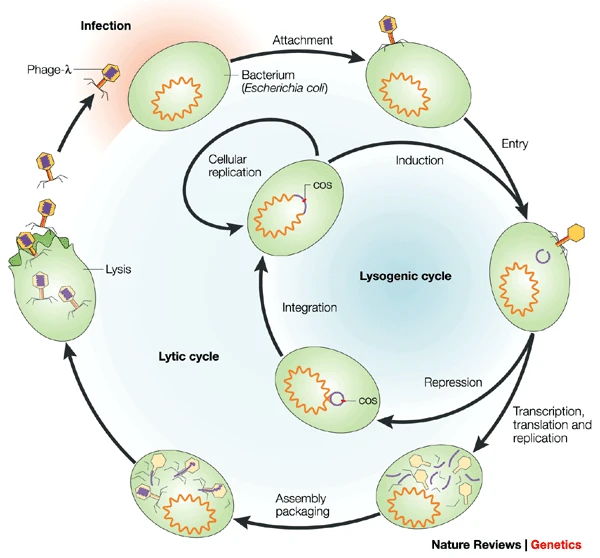
\includegraphics[width=0.5\linewidth]{Figures/phage_life_cycle.png}
    \caption{Life cycle of a phage, inside and outside a bacteria cell.}
    \label{fig:phage_life_cycle}
\end{figure}